\documentclass[tikz]{standalone}
\usetikzlibrary{arrows}
\begin{document}
%%%
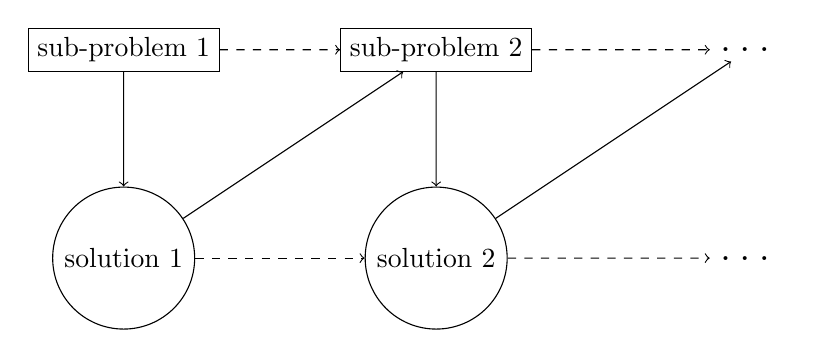
\begin{tikzpicture}[y=0.80pt, x=0.8pt,xscale=.75,yscale=.75]
\begin{scope}
 % nodi
  \node (p1) at ( 50bp,  150bp) [draw,rectangle] {sub-problem 1};
  \node (p2) at (200bp, 150bp) [draw,rectangle] {sub-problem 2};
  \node (p3) at (350bp, 150bp) [draw=none] {\LARGE\ldots};
  \node (s1) at ( 50bp,  50bp) [draw,circle] {solution 1};
  \node (s2) at (200bp,  50bp) [draw,circle] {solution 2};
  \node (s3) at (350bp,  50bp) [draw=none] {\LARGE\ldots};
 % archi
  \path[->,dashed] (p1) edge (p2);
  \path[->] (p1) edge (s1);
  \path[->] (s1) edge (p2);
  \path[->,dashed] (s1) edge (s2);
  \path[->,dashed] (p2) edge (p3);
  \path[->] (p2) edge (s2);
  \path[->] (s2) edge (p3);
  \path[->,dashed] (s2) edge (s3);
\end{scope}
\end{tikzpicture}
%%%
\end{document}